\chapter{Einleitung}
In diesem Kapitel möchten wir ein wenig Hintergrundwissen im Bereich der Computergrafik vorstellen. Eine kurze Geschichte über ein trabendes Pferd und eine skurrile Teekanne wird hier beschrieben.

\section{Geschichte}

\subsubsection{Eadweard Muybridge}
Um die erste Animation in der Geschichte zu finden müssen wir ins Jahr 1872. 
Eadweard Muybridge (geboren: 9. April 1830 in Kingston upon Thames, England; gestorben: 8. Mai 1904 ebenda) 
ein britischer Fotograf und Pionier der Fototechnik, bekam als Auftrag die 
Beinstellungen eines trabenden Pferdes zu bestimmen. \\
Muybridge meisterte die Aufgabe indem er mit 12, 24 und 36 sukzessive auslösenden Fotoapparaten 
arbeitete und somit die Serienfotografie gebar. Natürlich war das 
vergleichsweise zu heute ein schwieriges unterfangen, das Pferd löste auf 
einer Pferderennbahn gespannte Zugdrähte aus, welche wiederum die elektrisch 
betriebenen Hochgeschwindigkeitsblenden der Fotoapparate auslösten. So wurde 
erstmals der sichtbare Beweis erbracht, dass sich beim galoppierenden Pferd 
bei gewisser Zeit alle vier Beine in der Luft befinden.\\

\begin{figure}[htbp]
\center
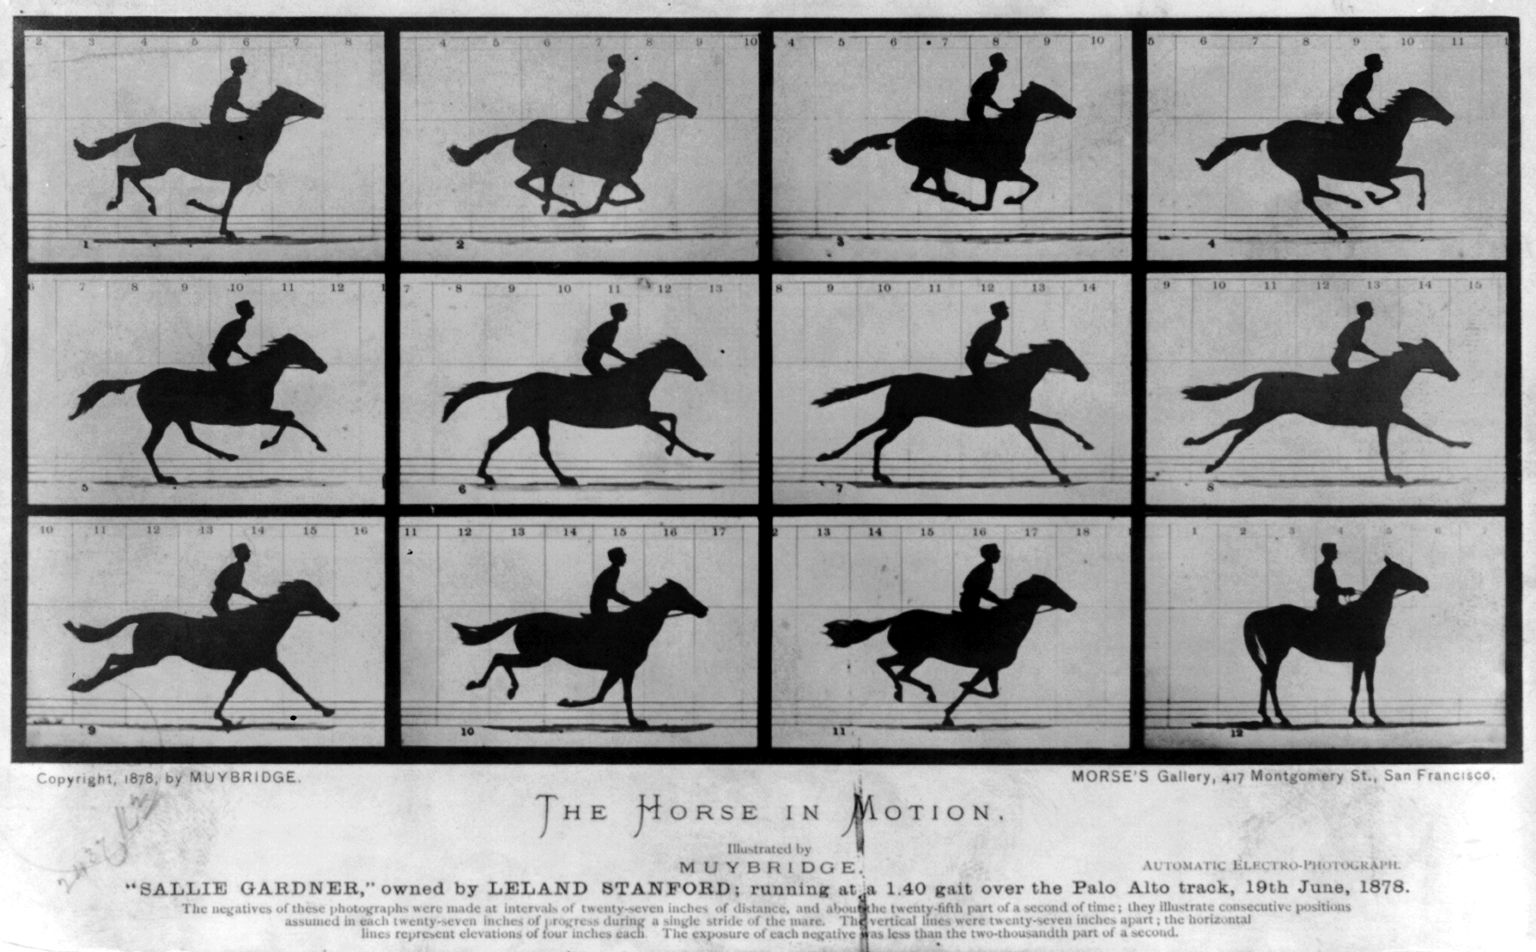
\includegraphics[scale=0.25]{include/The_Horse_in_Motion.jpg}
\caption{galoppierendes Pferd}
\end{figure}
Auf dem 2. und 3. Bild kann man gut erkennen, dass alle Beine gegen die Mitte gebogen und in der Luft sind. Eine weitere Erkenntnis ist auch, dass nie mehr als 2 Beine des Pferdes den Boden berühren. 

\subsubsection{Utah-Teekanne}

Zu jeder Computergrafik gehört selbstverständlich ein 3D-Modell. Eines der ältesten und berühmtesten 3D-Modelle ist die Utah-Teekanne (engl. Utah-Teapot). Hierbei handelt es sich um ein Oberflächenmodell einer Teekanne, bei der der Innenraum nicht modeliert wurde. 1975 entwickelte Martin Newell sie im Rahmen einer Forschungsarbeit an der Univeristät von Utah. \\
Als er nach einem Gebrauchsgegenstand für seine Arbeit suchte, fand er die Melitta-Teekanne seiner Frau für geeignet. In Computerzeitschriften wurde über die Jahre immer wieder das Modell übernommen und regelmässig Varianten der Teekanne präsentiert. Mittlerweile wurde es zu einer Art Running Gag in der Computergrafikszene und kommt beispielsweise ``versteckt'' in den Animationsfilmen Toy Story und Die Monster AG vor. Selbst 3D-Animations-Programme wie 3d Studio Max verwenden die Teekanne als Grundkonstruktionsobjekt. \\ 
Selbstverständlich nimmt die 3d-Modelierung ein grosser Teil in der Computerspielewelt ein. Jedoch möchten wir uns von diesem Teilgebiet differenzieren und die Animation und Bewegungen in Computerspielen genauer betrachten und erläutern.

\begin{figure}[htbp]
\center
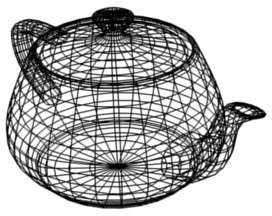
\includegraphics[scale=0.5]{include/teapot.png}
\caption{Utah-Teekanna}
\end{figure}

\section{Bildfrequenz}
Die Bildfrequenz ist ein Begriff aus der Film- und Videotechnik. Sie bezeichnet die Anzahl der Einzelbilder, die in einem Zeitraum aufgenommen werden. Die Bildfrequenz wird auch mit fps abgekürzt (für das englische Frames per Second).\\
Das menschliche Gehirn nimmt ab etwa 14 bis 16 aufeinander folgende Bildern pro Sekunde Bilder als bewegte Szene wahr.
Zur Stummfilmzeit wurden die Filme mit 16fps erzeugt. Später mit der Einführung des Tonfilms wurde die Bildfrequenz auf 24fps festgelegt, da die Tonqualität bei 16fps nicht ausreichte.

